\documentclass[11pt, a4paper, titlepage, block]{article}
\usepackage{listings}
\hyphenpenalty=10000

\usepackage{graphicx}
\begin{document}
\begin{titlepage}

\newcommand{\HRule}{\rule{\linewidth}{0.5mm}} % Defines a new command for the horizontal lines, change thickness here

\center % Center everything on the page
 
%----------------------------------------------------------------------------------------
%	HEADING SECTIONS
%----------------------------------------------------------------------------------------

\textsc{\LARGE Universita}\\[1.5cm] % Name of your university/college
\textsc{\Large applied computer science}\\[0.5cm] % Major heading such as course name
\textsc{\large Algoritmi e Strutture Dati}\\[0.5cm] % Minor heading such as course title

%----------------------------------------------------------------------------------------
%	TITLE SECTION
%----------------------------------------------------------------------------------------


\HRule \\[0.4cm]
{ \huge \bfseries Report}\\[0.2cm] % Title of your document
\HRule \\[0.4cm]
\textsc{\large Project for the 2013/2014 summer session}
\\[0.5cm]
%----------------------------------------------------------------------------------------
%	AUTHOR SECTION
%----------------------------------------------------------------------------------------

\begin{minipage}{\textwidth}
\begin{flushleft}
\emph{Student:}\\
Julian \textsc{Sparber}\\ % Your name
matric no: 260324
\end{flushleft}
\end{minipage}

\begin{minipage}{\textwidth}
\begin{flushright}
\emph{Lecturer:} \\
Valerio \textsc{Freschi} % Supervisor's Name
\end{flushright}
\end{minipage}\\[11cm]

%----------------------------------------------------------------------------------------
%	DATE SECTION
%----------------------------------------------------------------------------------------

{\large \today}\\[10cm] % Date, change the \today to a set date if you want to be precise

%----------------------------------------------------------------------------------------
%	LOGO SECTION
%----------------------------------------------------------------------------------------

%\includegraphics{Logo}\\[1cm] % Include a department/university logo - this will require the graphicx package
 
%----------------------------------------------------------------------------------------

\newpage

\end{titlepage}

\section{Specifica del problema}
	Si supponga di elaborare i dati relativi ad un grafo. Le informazioni associate al problema siano: un insieme di vertici (con nomi specifcati da stringhe prive di spazi) e un insieme di archi caratterizzati da una tripla di distanze d1, d2, d3 (una tripla di numeri reali).
	\subsection{}
	Acquisisce da file le informazioni relative al grafo. Il formato del file \`{e} del tipo:\\
	\begin{tabular}{|c|c|c|c|c|}
\hline
	{\textless}No. totale dei vertici{\textgreater} & & & & \\
\hline
	{\textless}No. di vertici collegati al vertice A{\textgreater} & & & & \\
\hline
	{\textless}vertice\_A{\textgreater} & {\textless}vertice\_B{\textgreater} & {\textless}d1{\textgreater} & {\textless}d2{\textgreater} & {\textless}d3{\textgreater}\\
\hline
	{\textless}vertice\_A{\textgreater} & {\textless}vertice\_M{\textgreater} & {\textless}d1{\textgreater} & {\textless}d2{\textgreater} & {\textless}d3{\textgreater}\\
\hline
	... & & & &\\
\hline
	{\textless}vertice\_A{\textgreater} & {\textless}vertice\_Z{\textgreater} & {\textless}d1{\textgreater} & {\textless}d2{\textgreater} & {\textless}d3{\textgreater}\\
\hline
	{\textless}No. di vertici collegati al vertice B{\textgreater} & & & &\\
\hline
	{\textless}vertice\_B{\textgreater} & {\textless}vertice\_C{\textgreater} & {\textless}d1{\textgreater} & {\textless}d2{\textgreater} & {\textless}d3{\textgreater}\\
\hline
	{\textless}vertice\_B{\textgreater} & {\textless}vertice\_X{\textgreater} & {\textless}d1{\textgreater} & {\textless}d2{\textgreater} & {\textless}d3{\textgreater}\\
\hline
	... & & & &\\
\hline
\end{tabular}
	\subsection{}
	Inserisce i dati acquisiti in una opportuna struttura dati.
	\subsection{}
	Dati un vertice sorgente, uno destinazione e una tipologia di distanze (d1 oppure d2 oppure d3) inseriti dall’utente, calcola il percorso pi\`{u} breve tra sorgente e destinazione, mostrando a
monitor tale percorso e la relativa distanza.
	\subsection{}
	Dato un vertice specificato dall’utente, calcola la media e la mediana della distanze minime che separano tale vertice da tutti gli altri vertici del grafo, in base alle tipologie di distanza d1, d2 e d3.\\ \\
	Per quanto riguarda l’analisi teorica si devono studiare le complessit\`{a} degli algoritmi di acquisizione del file (punto 2), calcolo del percorso pi\`{u} breve tra due vertici (punto 3) e calcolo di media e mediana (punto 4).\\
	Per quanto riguarda il punto 4 si deve anche verificare sperimentalmente la complessit\`{a} delcalcolo di media e mediana, generando casualmente una sequenza di distanze (di N numeri reali) da fornire come input all’algoritmo per valori crescenti di N.

	\newpage
\section{Progettazione dell problema}
Ogni carattere letto dal file viene direttamente verificato se \`{e} ammesso. Il nodo e l'arco presso da ogni riga viene salvato in una struttura dinamica di tipo: \\
\{\\
\indent nome del nodo,\\
\indent archi del nodo,\\
\indent minima distanza,\\
\indent parente del nodo,\\
\indent nodo successivo; \\
\}\\
dove i archi sono salvati in una struttura di tipo:\\
\{\\
  nome del nodo di destinazione,\\
  nodo di destinazione,\\
  la tripla della distanza,\\
  arco successivo;\\
\}\\
Un vertice sorgente, un vertice destinazione e una tipologia di distanze (d1 oppure d2 oppure d3) viene chiesto al utente.\\
In questo grafo si tratta di distanze quindi è una buona occasione di aspettare che no chi sono dei archi di peso negativo. Ne consegue che l' algoritmo di Dijkstra è una buona scelta.\\
La mediana è calcolato con quickselect, un algoritmo randomizzato che trova il k-esimo elemento di una struttura disordinata di grandezza n eseguendo O( n$^2$ ) confronti nel caso peggiore e O(n) nel caso ottimo. Quickselect è semplice da implementare è se ben implementata in pratica un po più veloce di heapselect.\\
Al utente viene mostrato il percorso pi\`{u} breve tra sorgente e destinazione, la media e la mediana della distanze minime che separano tale vertice da tutti gli altri vertici del grafo
	\newpage
\section{Valutazione della complessit\`{a} del programma}
Essendo che l' algoritmo in lavora si applica su strutture del tipo grafo, la complessità verrà espressa in 
funzione del numero di vertici e di archi del grafo stesso. A questo scopo verrà indicato con $|$V$|$ il 
numero di vertici e con $|$E$|$ (edges) il numero di tutti gli archi.\\
\\
La complessità del algoritmo di acquisizione:\\
\indent T($|$V$|$, $|$E$|$) = 1+ $|$V$|$ + $|$E$|$ = O($|$V$|$ + $|$E$|$)\\
La complessità del algoritmo per calcolare il percorso pi\`{u} breve tra due vertici(Algoritmo di Dijkstra):\\
\indent T ($|$V $|$, $|$E$|$) = O($|$V $|$ · log $|$V $|$ + $|$E$|$)\\
La complessità del algoritmo per calcolare la media:\\
\indent T($|$V$|$, $|$E$|$) = O($|$V$|$)\\
La complessità del algoritmo per calcolare la mediana(quickselect):\\
\indent Caso ottimo:\\
\indent \indent T($|$V$|$, $|$E$|$) = $|$V$|$ + $|$V$|$ + T($|$V$|$ / 2) = O($|$V$|$)\\
\indent Caso pessimo:\\
\indent \indent T($|$V$|$, $|$E$|$) = $|$V$|$ + $|$V$|$ + T($|$V$|$ - 1) = O($|$V$|$2)\\
	\newpage
\section{Valutazione sperimentalmente della complessit\`{a} del calcolo di media e mediana}
Si vede anche nella valutazione sperimentale la complessit\`{a} O($|$V$|$) del calcolo della media.
\begin{figure}[htp]
\centering
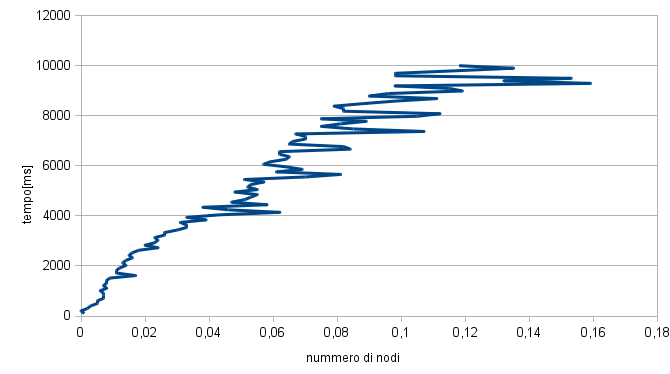
\includegraphics[scale=0.80]{img/calcolo_media.png}
\caption{complessit\`{a} del calcolo di media}
\end{figure}
\newpage
Anche l'risultato dalla valutazione sperimentale del calcolo della mediana non porta inaspettato. Qui si vede l'confronto dal calcolo di media e di mediana. La complessit\`{a} varia molto perch\`{e} quickselect \`{e} randomizzato quindi dipende molto dalla partenza.
\begin{figure}[htp]
\centering
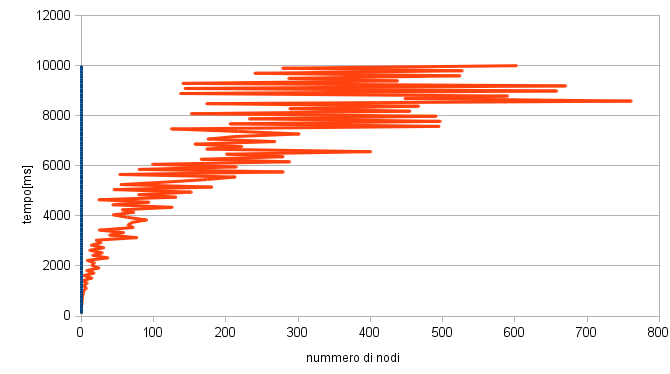
\includegraphics[scale=0.80]{img/calcolo_mediana.png}
\caption{complessit\`{a} del calcolo di media(blue) e mediana(rosso)}
\end{figure}

\end{document}
